
\documentclass{article}

\usepackage{pgf}
\usepackage{array}
\usepackage{caption}
\usepackage{subcaption}
\usepackage{geometry}
\usepackage{multirow}
\usepackage{pdflscape}
\usepackage{booktabs}
\usepackage{graphicx}
\usepackage[utf8]{inputenc}
\usepackage{pgfplots}
\usepgfplotslibrary{groupplots,dateplot}
\usetikzlibrary{patterns,shapes.arrows}
\pgfplotsset{compat=newest}


\begin{document}
\newgeometry{margin=1in}


\begin{table}[h!tbp]
  \centering
  \renewcommand{\arraystretch}{1.2}
  \begin{tabular}{lccc}
    \toprule
    \multirow{2}{*}{\textbf{Metrics}} & \multicolumn{3}{c}{\textbf{Scores}} \\
    \cmidrule(lr){2-4}
    & \textbf{Human}& \textbf{Yeast} \\
    \midrule
    \textbf{Accuracy} & 0.80& 0.84 \\
    \textbf{Mathew's CC} & 0.60& 0.68 \\
    \textbf{Cohen's Kappa} & 0.60& 0.68 \\
    \textbf{Specificity} & 0.78& 0.78 \\
    \bottomrule
  \end{tabular}
  \caption{Classifier Metrics of all species}
\end{table}

\vspace{100pt}


\begin{table}[h!tbp]

\centering
\renewcommand{\arraystretch}{1.2}

\begin{tabular}{rcc}
  \toprule
  & \textbf{Predicted} $-ive$ & \textbf{Predicted} $+ive$ \\
  \midrule
  \textbf{Actual} $-ive$ & 78 & 22 \\
  \textbf{Actual} $+ive$ & 18 & 82 \\
  \bottomrule
\end{tabular}

\caption{Confusion Matrix for Human}
\end{table}


\begin{table}[h!tbp]

\centering
\renewcommand{\arraystretch}{1.2}

\begin{tabular}{rcc}
  \toprule
  & \textbf{Predicted} $-ive$ & \textbf{Predicted} $+ive$ \\
  \midrule
  \textbf{Actual} $-ive$ & 78 & 22 \\
  \textbf{Actual} $+ive$ & 10 & 90 \\
  \bottomrule
\end{tabular}

\caption{Confusion Matrix for Yeast}
\end{table}



\begin{table}[htbp]

\centering
\renewcommand{\arraystretch}{1.2}

\begin{tabular}{rcccc}
  \toprule
  & \textbf{Precision} & \textbf{Recall} & \textbf{F1-Score} & \textbf{Support} \\
  \midrule
  \textbf{0} & 0.81 & 0.81 & 0.81 & 0.81 \\
  \textbf{1} & 0.79 & 0.79 & 0.79 & 0.79 \\
  \textbf{Macro Avg} & 0.80 & 0.80 & 0.80 & 0.80 \\
  \textbf{Weighted Avg} & 0.80 & 0.80 & 0.80 & 0.80 \\
  \bottomrule
\end{tabular}

\caption{Classification Report for Human}
\end{table}


\begin{table}[htbp]

\centering
\renewcommand{\arraystretch}{1.2}

\begin{tabular}{rcccc}
  \toprule
  & \textbf{Precision} & \textbf{Recall} & \textbf{F1-Score} & \textbf{Support} \\
  \midrule
  \textbf{0} & 0.89 & 0.89 & 0.89 & 0.89 \\
  \textbf{1} & 0.80 & 0.80 & 0.80 & 0.80 \\
  \textbf{Macro Avg} & 0.84 & 0.84 & 0.84 & 0.84 \\
  \textbf{Weighted Avg} & 0.84 & 0.84 & 0.84 & 0.84 \\
  \bottomrule
\end{tabular}

\caption{Classification Report for Yeast}
\end{table}


\clearpage
\newgeometry{landscape, margin=0.25in}
\begin{landscape}


\begin{table}
  \begin{tabular}{ccc}
    % This file was created with tikzplotlib v0.10.1.
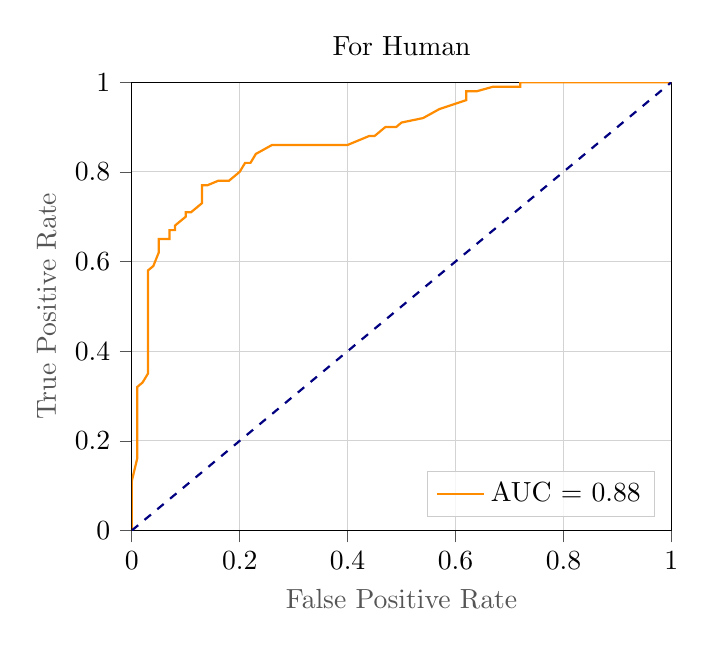
\begin{tikzpicture}

\definecolor{darkorange}{RGB}{255,140,0}
\definecolor{dimgray85}{RGB}{85,85,85}
\definecolor{lightgray}{RGB}{211,211,211}
\definecolor{lightgray204}{RGB}{204,204,204}
\definecolor{navy}{RGB}{0,0,128}

\begin{axis}[
legend cell align={left},
legend style={
  fill opacity=0.8,
  draw opacity=1,
  text opacity=1,
  at={(0.97,0.03)},
  anchor=south east,
  draw=lightgray204
},
tick align=outside,
tick pos=left,
title={For Human},
x grid style={lightgray},
xlabel=\textcolor{dimgray85}{False Positive Rate},
xmajorgrids,
xmin=0, xmax=1,
xtick style={color=dimgray85},
y grid style={lightgray},
ylabel=\textcolor{dimgray85}{True Positive Rate},
ymajorgrids,
ymin=0, ymax=1,
ytick style={color=dimgray85}
]
\addplot [thick, darkorange]
table {%
0 0
0 0.02
0 0.05
0 0.07
0 0.11
0.01 0.16
0.01 0.2
0.01 0.32
0.02 0.33
0.03 0.35
0.03 0.36
0.03 0.4
0.03 0.42
0.03 0.5
0.03 0.51
0.03 0.54
0.03 0.58
0.04 0.59
0.05 0.62
0.05 0.65
0.07 0.65
0.07 0.67
0.08 0.67
0.08 0.68
0.1 0.7
0.1 0.71
0.11 0.71
0.13 0.73
0.13 0.77
0.14 0.77
0.16 0.78
0.18 0.78
0.2 0.8
0.21 0.82
0.22 0.82
0.23 0.84
0.26 0.86
0.27 0.86
0.31 0.86
0.32 0.86
0.34 0.86
0.4 0.86
0.44 0.88
0.45 0.88
0.47 0.9
0.49 0.9
0.5 0.91
0.54 0.92
0.57 0.94
0.62 0.96
0.62 0.98
0.64 0.98
0.67 0.99
0.72 0.99
0.72 1
0.73 1
0.76 1
0.78 1
0.79 1
0.83 1
0.85 1
0.87 1
0.9 1
0.93 1
0.97 1
1 1
};
\addlegendentry{AUC = 0.88}
\addplot [thick, navy, dashed, forget plot]
table {%
0 0
1 1
};
\end{axis}

\end{tikzpicture}
&% This file was created with tikzplotlib v0.10.1.
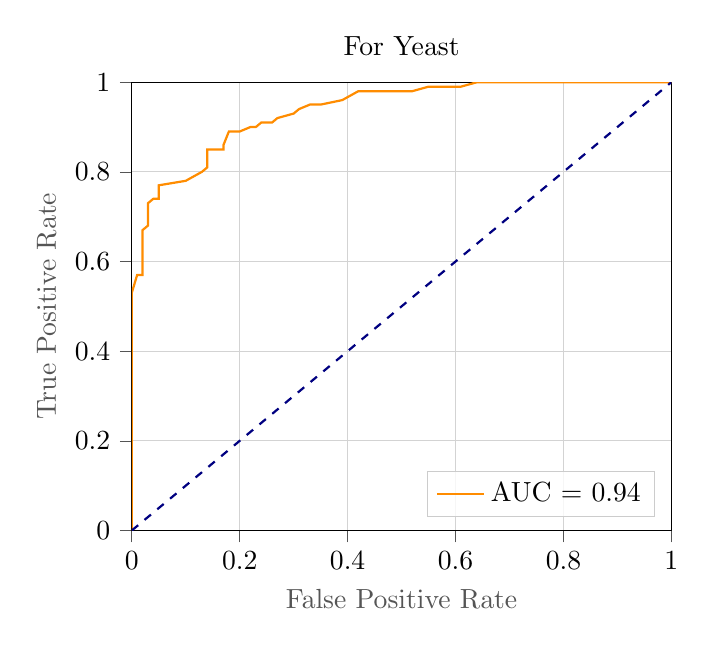
\begin{tikzpicture}

\definecolor{darkorange}{RGB}{255,140,0}
\definecolor{dimgray85}{RGB}{85,85,85}
\definecolor{lightgray}{RGB}{211,211,211}
\definecolor{lightgray204}{RGB}{204,204,204}
\definecolor{navy}{RGB}{0,0,128}

\begin{axis}[
legend cell align={left},
legend style={
  fill opacity=0.8,
  draw opacity=1,
  text opacity=1,
  at={(0.97,0.03)},
  anchor=south east,
  draw=lightgray204
},
tick align=outside,
tick pos=left,
title={For Yeast},
x grid style={lightgray},
xlabel=\textcolor{dimgray85}{False Positive Rate},
xmajorgrids,
xmin=0, xmax=1,
xtick style={color=dimgray85},
y grid style={lightgray},
ylabel=\textcolor{dimgray85}{True Positive Rate},
ymajorgrids,
ymin=0, ymax=1,
ytick style={color=dimgray85}
]
\addplot [thick, darkorange]
table {%
0 0
0 0.04
0 0.05
0 0.09
0 0.1
0 0.12
0 0.16
0 0.19
0 0.25
0 0.26
0 0.29
0 0.33
0 0.36
0 0.38
0 0.42
0 0.44
0 0.5
0 0.52
0 0.53
0.01 0.57
0.02 0.57
0.02 0.67
0.03 0.68
0.03 0.69
0.03 0.73
0.04 0.74
0.05 0.74
0.05 0.76
0.05 0.77
0.1 0.78
0.13 0.8
0.14 0.81
0.14 0.85
0.17 0.85
0.17 0.86
0.18 0.89
0.2 0.89
0.22 0.9
0.23 0.9
0.24 0.91
0.26 0.91
0.27 0.92
0.3 0.93
0.31 0.94
0.33 0.95
0.35 0.95
0.39 0.96
0.42 0.98
0.46 0.98
0.49 0.98
0.51 0.98
0.52 0.98
0.55 0.99
0.57 0.99
0.61 0.99
0.64 1
0.66 1
0.69 1
0.7 1
0.72 1
0.73 1
0.75 1
0.77 1
0.8 1
0.88 1
0.89 1
0.92 1
0.95 1
0.97 1
1 1
};
\addlegendentry{AUC = 0.94}
\addplot [thick, navy, dashed, forget plot]
table {%
0 0
1 1
};
\end{axis}

\end{tikzpicture}
 \\
  \end{tabular}
  \caption{Receiver operating characteristic (ROC) curves}
\end{table}


\begin{table}
  \begin{tabular}{ccc}
    % This file was created with tikzplotlib v0.10.1.
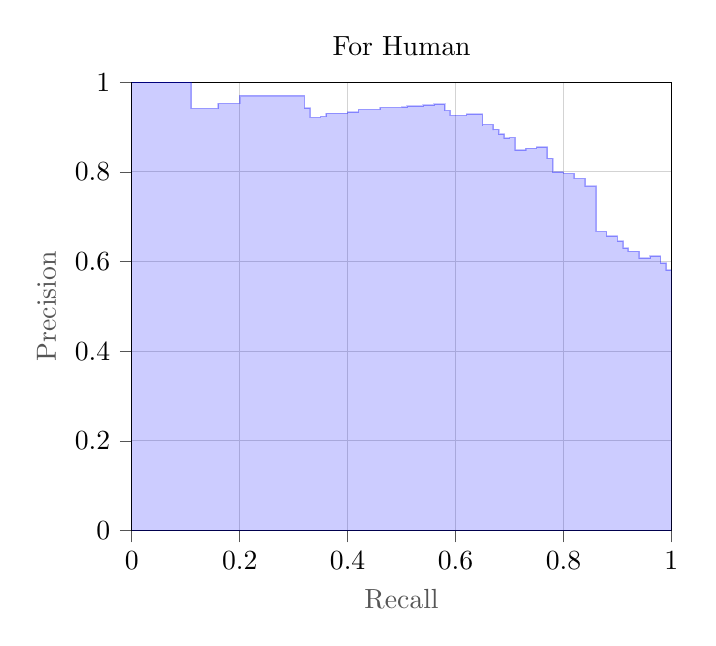
\begin{tikzpicture}

\definecolor{dimgray85}{RGB}{85,85,85}
\definecolor{lightgray}{RGB}{211,211,211}

\begin{axis}[
tick align=outside,
tick pos=left,
title={For Human},
x grid style={lightgray},
xlabel=\textcolor{dimgray85}{Recall},
xmajorgrids,
xmin=0, xmax=1,
xtick style={color=dimgray85},
y grid style={lightgray},
ylabel=\textcolor{dimgray85}{Precision},
ymajorgrids,
ymin=0, ymax=1,
ytick style={color=dimgray85}
]
\path [draw=blue, fill=blue, opacity=0.2, very thin]
(axis cs:1,0)
--(axis cs:1,0.5)
--(axis cs:1,0.5)
--(axis cs:1,0.50251256281407)
--(axis cs:1,0.50251256281407)
--(axis cs:1,0.505050505050505)
--(axis cs:1,0.505050505050505)
--(axis cs:1,0.50761421319797)
--(axis cs:1,0.50761421319797)
--(axis cs:1,0.512820512820513)
--(axis cs:1,0.512820512820513)
--(axis cs:1,0.518134715025907)
--(axis cs:1,0.518134715025907)
--(axis cs:1,0.526315789473684)
--(axis cs:1,0.526315789473684)
--(axis cs:1,0.529100529100529)
--(axis cs:1,0.529100529100529)
--(axis cs:1,0.531914893617021)
--(axis cs:1,0.531914893617021)
--(axis cs:1,0.53475935828877)
--(axis cs:1,0.53475935828877)
--(axis cs:1,0.540540540540541)
--(axis cs:1,0.540540540540541)
--(axis cs:1,0.543478260869565)
--(axis cs:1,0.543478260869565)
--(axis cs:1,0.546448087431694)
--(axis cs:1,0.546448087431694)
--(axis cs:1,0.552486187845304)
--(axis cs:1,0.552486187845304)
--(axis cs:1,0.558659217877095)
--(axis cs:1,0.558659217877095)
--(axis cs:1,0.561797752808989)
--(axis cs:1,0.561797752808989)
--(axis cs:1,0.568181818181818)
--(axis cs:1,0.568181818181818)
--(axis cs:1,0.578034682080925)
--(axis cs:1,0.578034682080925)
--(axis cs:1,0.581395348837209)
--(axis cs:0.99,0.581395348837209)
--(axis cs:0.99,0.578947368421053)
--(axis cs:0.99,0.578947368421053)
--(axis cs:0.99,0.596385542168675)
--(axis cs:0.98,0.596385542168675)
--(axis cs:0.98,0.604938271604938)
--(axis cs:0.98,0.604938271604938)
--(axis cs:0.98,0.6125)
--(axis cs:0.96,0.6125)
--(axis cs:0.96,0.607594936708861)
--(axis cs:0.94,0.607594936708861)
--(axis cs:0.94,0.622516556291391)
--(axis cs:0.92,0.622516556291391)
--(axis cs:0.92,0.63013698630137)
--(axis cs:0.91,0.63013698630137)
--(axis cs:0.91,0.645390070921986)
--(axis cs:0.9,0.645390070921986)
--(axis cs:0.9,0.647482014388489)
--(axis cs:0.9,0.647482014388489)
--(axis cs:0.9,0.656934306569343)
--(axis cs:0.88,0.656934306569343)
--(axis cs:0.88,0.661654135338346)
--(axis cs:0.88,0.661654135338346)
--(axis cs:0.88,0.666666666666667)
--(axis cs:0.86,0.666666666666667)
--(axis cs:0.86,0.682539682539683)
--(axis cs:0.86,0.682539682539683)
--(axis cs:0.86,0.699186991869919)
--(axis cs:0.86,0.699186991869919)
--(axis cs:0.86,0.716666666666667)
--(axis cs:0.86,0.716666666666667)
--(axis cs:0.86,0.728813559322034)
--(axis cs:0.86,0.728813559322034)
--(axis cs:0.86,0.735042735042735)
--(axis cs:0.86,0.735042735042735)
--(axis cs:0.86,0.761061946902655)
--(axis cs:0.86,0.761061946902655)
--(axis cs:0.86,0.767857142857143)
--(axis cs:0.84,0.767857142857143)
--(axis cs:0.84,0.785046728971963)
--(axis cs:0.82,0.785046728971963)
--(axis cs:0.82,0.788461538461538)
--(axis cs:0.82,0.788461538461538)
--(axis cs:0.82,0.796116504854369)
--(axis cs:0.8,0.796116504854369)
--(axis cs:0.8,0.8)
--(axis cs:0.78,0.8)
--(axis cs:0.78,0.8125)
--(axis cs:0.78,0.8125)
--(axis cs:0.78,0.821052631578947)
--(axis cs:0.78,0.821052631578947)
--(axis cs:0.78,0.829787234042553)
--(axis cs:0.77,0.829787234042553)
--(axis cs:0.77,0.846153846153846)
--(axis cs:0.77,0.846153846153846)
--(axis cs:0.77,0.855555555555556)
--(axis cs:0.75,0.855555555555556)
--(axis cs:0.75,0.852272727272727)
--(axis cs:0.73,0.852272727272727)
--(axis cs:0.73,0.848837209302326)
--(axis cs:0.71,0.848837209302326)
--(axis cs:0.71,0.865853658536585)
--(axis cs:0.71,0.865853658536585)
--(axis cs:0.71,0.876543209876543)
--(axis cs:0.7,0.876543209876543)
--(axis cs:0.7,0.875)
--(axis cs:0.69,0.875)
--(axis cs:0.69,0.884615384615385)
--(axis cs:0.68,0.884615384615385)
--(axis cs:0.68,0.894736842105263)
--(axis cs:0.67,0.894736842105263)
--(axis cs:0.67,0.893333333333333)
--(axis cs:0.67,0.893333333333333)
--(axis cs:0.67,0.905405405405405)
--(axis cs:0.65,0.905405405405405)
--(axis cs:0.65,0.902777777777778)
--(axis cs:0.65,0.902777777777778)
--(axis cs:0.65,0.928571428571429)
--(axis cs:0.62,0.928571428571429)
--(axis cs:0.62,0.925373134328358)
--(axis cs:0.59,0.925373134328358)
--(axis cs:0.59,0.936507936507937)
--(axis cs:0.58,0.936507936507937)
--(axis cs:0.58,0.950819672131147)
--(axis cs:0.56,0.950819672131147)
--(axis cs:0.56,0.949152542372881)
--(axis cs:0.54,0.949152542372881)
--(axis cs:0.54,0.947368421052632)
--(axis cs:0.51,0.947368421052632)
--(axis cs:0.51,0.944444444444444)
--(axis cs:0.5,0.944444444444444)
--(axis cs:0.5,0.943396226415094)
--(axis cs:0.46,0.943396226415094)
--(axis cs:0.46,0.938775510204082)
--(axis cs:0.42,0.938775510204082)
--(axis cs:0.42,0.933333333333333)
--(axis cs:0.4,0.933333333333333)
--(axis cs:0.4,0.930232558139535)
--(axis cs:0.36,0.930232558139535)
--(axis cs:0.36,0.923076923076923)
--(axis cs:0.35,0.923076923076923)
--(axis cs:0.35,0.921052631578947)
--(axis cs:0.33,0.921052631578947)
--(axis cs:0.33,0.942857142857143)
--(axis cs:0.32,0.942857142857143)
--(axis cs:0.32,0.96969696969697)
--(axis cs:0.2,0.96969696969697)
--(axis cs:0.2,0.952380952380952)
--(axis cs:0.16,0.952380952380952)
--(axis cs:0.16,0.941176470588235)
--(axis cs:0.11,0.941176470588235)
--(axis cs:0.11,1)
--(axis cs:0.09,1)
--(axis cs:0.09,1)
--(axis cs:0.07,1)
--(axis cs:0.07,1)
--(axis cs:0.06,1)
--(axis cs:0.06,1)
--(axis cs:0.05,1)
--(axis cs:0.05,1)
--(axis cs:0.02,1)
--(axis cs:0.02,1)
--(axis cs:0,1)
--(axis cs:0,1)
--(axis cs:0,0)
--(axis cs:0,0)
--(axis cs:0,0)
--(axis cs:0.02,0)
--(axis cs:0.02,0)
--(axis cs:0.05,0)
--(axis cs:0.05,0)
--(axis cs:0.06,0)
--(axis cs:0.06,0)
--(axis cs:0.07,0)
--(axis cs:0.07,0)
--(axis cs:0.09,0)
--(axis cs:0.09,0)
--(axis cs:0.11,0)
--(axis cs:0.11,0)
--(axis cs:0.16,0)
--(axis cs:0.16,0)
--(axis cs:0.2,0)
--(axis cs:0.2,0)
--(axis cs:0.32,0)
--(axis cs:0.32,0)
--(axis cs:0.33,0)
--(axis cs:0.33,0)
--(axis cs:0.35,0)
--(axis cs:0.35,0)
--(axis cs:0.36,0)
--(axis cs:0.36,0)
--(axis cs:0.4,0)
--(axis cs:0.4,0)
--(axis cs:0.42,0)
--(axis cs:0.42,0)
--(axis cs:0.46,0)
--(axis cs:0.46,0)
--(axis cs:0.5,0)
--(axis cs:0.5,0)
--(axis cs:0.51,0)
--(axis cs:0.51,0)
--(axis cs:0.54,0)
--(axis cs:0.54,0)
--(axis cs:0.56,0)
--(axis cs:0.56,0)
--(axis cs:0.58,0)
--(axis cs:0.58,0)
--(axis cs:0.59,0)
--(axis cs:0.59,0)
--(axis cs:0.62,0)
--(axis cs:0.62,0)
--(axis cs:0.65,0)
--(axis cs:0.65,0)
--(axis cs:0.65,0)
--(axis cs:0.65,0)
--(axis cs:0.67,0)
--(axis cs:0.67,0)
--(axis cs:0.67,0)
--(axis cs:0.67,0)
--(axis cs:0.68,0)
--(axis cs:0.68,0)
--(axis cs:0.69,0)
--(axis cs:0.69,0)
--(axis cs:0.7,0)
--(axis cs:0.7,0)
--(axis cs:0.71,0)
--(axis cs:0.71,0)
--(axis cs:0.71,0)
--(axis cs:0.71,0)
--(axis cs:0.73,0)
--(axis cs:0.73,0)
--(axis cs:0.75,0)
--(axis cs:0.75,0)
--(axis cs:0.77,0)
--(axis cs:0.77,0)
--(axis cs:0.77,0)
--(axis cs:0.77,0)
--(axis cs:0.78,0)
--(axis cs:0.78,0)
--(axis cs:0.78,0)
--(axis cs:0.78,0)
--(axis cs:0.78,0)
--(axis cs:0.78,0)
--(axis cs:0.8,0)
--(axis cs:0.8,0)
--(axis cs:0.82,0)
--(axis cs:0.82,0)
--(axis cs:0.82,0)
--(axis cs:0.82,0)
--(axis cs:0.84,0)
--(axis cs:0.84,0)
--(axis cs:0.86,0)
--(axis cs:0.86,0)
--(axis cs:0.86,0)
--(axis cs:0.86,0)
--(axis cs:0.86,0)
--(axis cs:0.86,0)
--(axis cs:0.86,0)
--(axis cs:0.86,0)
--(axis cs:0.86,0)
--(axis cs:0.86,0)
--(axis cs:0.86,0)
--(axis cs:0.86,0)
--(axis cs:0.86,0)
--(axis cs:0.86,0)
--(axis cs:0.88,0)
--(axis cs:0.88,0)
--(axis cs:0.88,0)
--(axis cs:0.88,0)
--(axis cs:0.9,0)
--(axis cs:0.9,0)
--(axis cs:0.9,0)
--(axis cs:0.9,0)
--(axis cs:0.91,0)
--(axis cs:0.91,0)
--(axis cs:0.92,0)
--(axis cs:0.92,0)
--(axis cs:0.94,0)
--(axis cs:0.94,0)
--(axis cs:0.96,0)
--(axis cs:0.96,0)
--(axis cs:0.98,0)
--(axis cs:0.98,0)
--(axis cs:0.98,0)
--(axis cs:0.98,0)
--(axis cs:0.99,0)
--(axis cs:0.99,0)
--(axis cs:0.99,0)
--(axis cs:0.99,0)
--(axis cs:1,0)
--(axis cs:1,0)
--(axis cs:1,0)
--(axis cs:1,0)
--(axis cs:1,0)
--(axis cs:1,0)
--(axis cs:1,0)
--(axis cs:1,0)
--(axis cs:1,0)
--(axis cs:1,0)
--(axis cs:1,0)
--(axis cs:1,0)
--(axis cs:1,0)
--(axis cs:1,0)
--(axis cs:1,0)
--(axis cs:1,0)
--(axis cs:1,0)
--(axis cs:1,0)
--(axis cs:1,0)
--(axis cs:1,0)
--(axis cs:1,0)
--(axis cs:1,0)
--(axis cs:1,0)
--(axis cs:1,0)
--(axis cs:1,0)
--(axis cs:1,0)
--(axis cs:1,0)
--(axis cs:1,0)
--(axis cs:1,0)
--(axis cs:1,0)
--(axis cs:1,0)
--(axis cs:1,0)
--(axis cs:1,0)
--(axis cs:1,0)
--(axis cs:1,0)
--(axis cs:1,0)
--(axis cs:1,0)
--cycle;

\addplot [semithick, blue, const plot mark left, opacity=0.2]
table {%
1 0.5
1 0.50251256281407
1 0.505050505050505
1 0.50761421319797
1 0.512820512820513
1 0.518134715025907
1 0.526315789473684
1 0.529100529100529
1 0.531914893617021
1 0.53475935828877
1 0.540540540540541
1 0.543478260869565
1 0.546448087431694
1 0.552486187845304
1 0.558659217877095
1 0.561797752808989
1 0.568181818181818
1 0.578034682080925
1 0.581395348837209
0.99 0.578947368421053
0.99 0.596385542168675
0.98 0.604938271604938
0.98 0.6125
0.96 0.607594936708861
0.94 0.622516556291391
0.92 0.63013698630137
0.91 0.645390070921986
0.9 0.647482014388489
0.9 0.656934306569343
0.88 0.661654135338346
0.88 0.666666666666667
0.86 0.682539682539683
0.86 0.699186991869919
0.86 0.716666666666667
0.86 0.728813559322034
0.86 0.735042735042735
0.86 0.761061946902655
0.86 0.767857142857143
0.84 0.785046728971963
0.82 0.788461538461538
0.82 0.796116504854369
0.8 0.8
0.78 0.8125
0.78 0.821052631578947
0.78 0.829787234042553
0.77 0.846153846153846
0.77 0.855555555555556
0.75 0.852272727272727
0.73 0.848837209302326
0.71 0.865853658536585
0.71 0.876543209876543
0.7 0.875
0.69 0.884615384615385
0.68 0.894736842105263
0.67 0.893333333333333
0.67 0.905405405405405
0.65 0.902777777777778
0.65 0.928571428571429
0.62 0.925373134328358
0.59 0.936507936507937
0.58 0.950819672131147
0.56 0.949152542372881
0.54 0.947368421052632
0.51 0.944444444444444
0.5 0.943396226415094
0.46 0.938775510204082
0.42 0.933333333333333
0.4 0.930232558139535
0.36 0.923076923076923
0.35 0.921052631578947
0.33 0.942857142857143
0.32 0.96969696969697
0.2 0.952380952380952
0.16 0.941176470588235
0.11 1
0.09 1
0.07 1
0.06 1
0.05 1
0.02 1
0 1
};
\end{axis}

\end{tikzpicture}
&% This file was created with tikzplotlib v0.10.1.
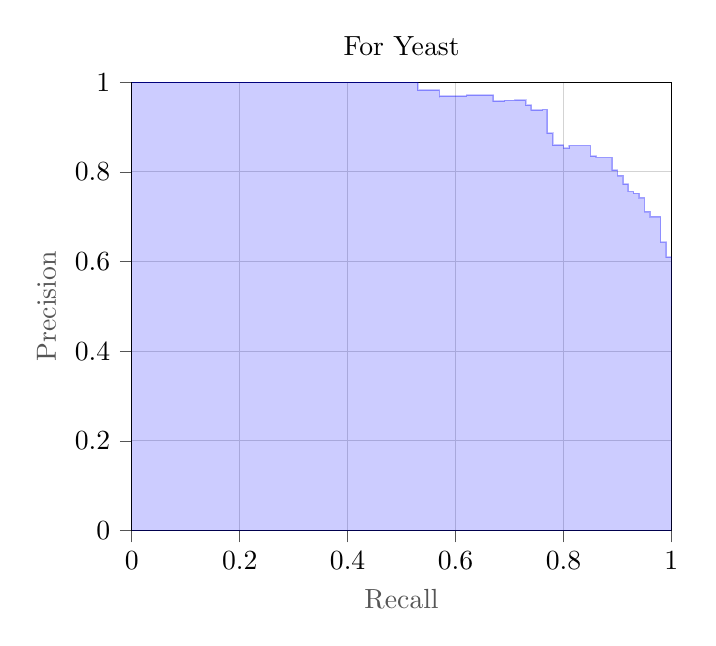
\begin{tikzpicture}

\definecolor{dimgray85}{RGB}{85,85,85}
\definecolor{lightgray}{RGB}{211,211,211}

\begin{axis}[
tick align=outside,
tick pos=left,
title={For Yeast},
x grid style={lightgray},
xlabel=\textcolor{dimgray85}{Recall},
xmajorgrids,
xmin=0, xmax=1,
xtick style={color=dimgray85},
y grid style={lightgray},
ylabel=\textcolor{dimgray85}{Precision},
ymajorgrids,
ymin=0, ymax=1,
ytick style={color=dimgray85}
]
\path [draw=blue, fill=blue, opacity=0.2, very thin]
(axis cs:1,0)
--(axis cs:1,0.5)
--(axis cs:1,0.5)
--(axis cs:1,0.50251256281407)
--(axis cs:1,0.50251256281407)
--(axis cs:1,0.505050505050505)
--(axis cs:1,0.505050505050505)
--(axis cs:1,0.50761421319797)
--(axis cs:1,0.50761421319797)
--(axis cs:1,0.512820512820513)
--(axis cs:1,0.512820512820513)
--(axis cs:1,0.515463917525773)
--(axis cs:1,0.515463917525773)
--(axis cs:1,0.518134715025907)
--(axis cs:1,0.518134715025907)
--(axis cs:1,0.520833333333333)
--(axis cs:1,0.520833333333333)
--(axis cs:1,0.529100529100529)
--(axis cs:1,0.529100529100529)
--(axis cs:1,0.531914893617021)
--(axis cs:1,0.531914893617021)
--(axis cs:1,0.537634408602151)
--(axis cs:1,0.537634408602151)
--(axis cs:1,0.543478260869565)
--(axis cs:1,0.543478260869565)
--(axis cs:1,0.549450549450549)
--(axis cs:1,0.549450549450549)
--(axis cs:1,0.555555555555556)
--(axis cs:1,0.555555555555556)
--(axis cs:1,0.564971751412429)
--(axis cs:1,0.564971751412429)
--(axis cs:1,0.568181818181818)
--(axis cs:1,0.568181818181818)
--(axis cs:1,0.571428571428571)
--(axis cs:1,0.571428571428571)
--(axis cs:1,0.578034682080925)
--(axis cs:1,0.578034682080925)
--(axis cs:1,0.581395348837209)
--(axis cs:1,0.581395348837209)
--(axis cs:1,0.588235294117647)
--(axis cs:1,0.588235294117647)
--(axis cs:1,0.591715976331361)
--(axis cs:1,0.591715976331361)
--(axis cs:1,0.602409638554217)
--(axis cs:1,0.602409638554217)
--(axis cs:1,0.609756097560976)
--(axis cs:0.99,0.609756097560976)
--(axis cs:0.99,0.61875)
--(axis cs:0.99,0.61875)
--(axis cs:0.99,0.634615384615385)
--(axis cs:0.99,0.634615384615385)
--(axis cs:0.99,0.642857142857143)
--(axis cs:0.98,0.642857142857143)
--(axis cs:0.98,0.653333333333333)
--(axis cs:0.98,0.653333333333333)
--(axis cs:0.98,0.657718120805369)
--(axis cs:0.98,0.657718120805369)
--(axis cs:0.98,0.666666666666667)
--(axis cs:0.98,0.666666666666667)
--(axis cs:0.98,0.680555555555556)
--(axis cs:0.98,0.680555555555556)
--(axis cs:0.98,0.7)
--(axis cs:0.96,0.7)
--(axis cs:0.96,0.711111111111111)
--(axis cs:0.95,0.711111111111111)
--(axis cs:0.95,0.730769230769231)
--(axis cs:0.95,0.730769230769231)
--(axis cs:0.95,0.736434108527132)
--(axis cs:0.95,0.736434108527132)
--(axis cs:0.95,0.7421875)
--(axis cs:0.94,0.7421875)
--(axis cs:0.94,0.752)
--(axis cs:0.93,0.752)
--(axis cs:0.93,0.75609756097561)
--(axis cs:0.92,0.75609756097561)
--(axis cs:0.92,0.773109243697479)
--(axis cs:0.91,0.773109243697479)
--(axis cs:0.91,0.777777777777778)
--(axis cs:0.91,0.777777777777778)
--(axis cs:0.91,0.791304347826087)
--(axis cs:0.9,0.791304347826087)
--(axis cs:0.9,0.79646017699115)
--(axis cs:0.9,0.79646017699115)
--(axis cs:0.9,0.803571428571429)
--(axis cs:0.89,0.803571428571429)
--(axis cs:0.89,0.81651376146789)
--(axis cs:0.89,0.81651376146789)
--(axis cs:0.89,0.831775700934579)
--(axis cs:0.86,0.831775700934579)
--(axis cs:0.86,0.83495145631068)
--(axis cs:0.85,0.83495145631068)
--(axis cs:0.85,0.833333333333333)
--(axis cs:0.85,0.833333333333333)
--(axis cs:0.85,0.858585858585859)
--(axis cs:0.81,0.858585858585859)
--(axis cs:0.81,0.852631578947368)
--(axis cs:0.8,0.852631578947368)
--(axis cs:0.8,0.860215053763441)
--(axis cs:0.78,0.860215053763441)
--(axis cs:0.78,0.886363636363636)
--(axis cs:0.77,0.886363636363636)
--(axis cs:0.77,0.939024390243902)
--(axis cs:0.76,0.939024390243902)
--(axis cs:0.76,0.938271604938272)
--(axis cs:0.74,0.938271604938272)
--(axis cs:0.74,0.936708860759494)
--(axis cs:0.74,0.936708860759494)
--(axis cs:0.74,0.948717948717949)
--(axis cs:0.73,0.948717948717949)
--(axis cs:0.73,0.960526315789474)
--(axis cs:0.71,0.960526315789474)
--(axis cs:0.71,0.959459459459459)
--(axis cs:0.69,0.959459459459459)
--(axis cs:0.69,0.958333333333333)
--(axis cs:0.68,0.958333333333333)
--(axis cs:0.68,0.957746478873239)
--(axis cs:0.67,0.957746478873239)
--(axis cs:0.67,0.971014492753623)
--(axis cs:0.62,0.971014492753623)
--(axis cs:0.62,0.96875)
--(axis cs:0.57,0.96875)
--(axis cs:0.57,0.966101694915254)
--(axis cs:0.57,0.966101694915254)
--(axis cs:0.57,0.982758620689655)
--(axis cs:0.53,0.982758620689655)
--(axis cs:0.53,1)
--(axis cs:0.52,1)
--(axis cs:0.52,1)
--(axis cs:0.5,1)
--(axis cs:0.5,1)
--(axis cs:0.47,1)
--(axis cs:0.47,1)
--(axis cs:0.44,1)
--(axis cs:0.44,1)
--(axis cs:0.42,1)
--(axis cs:0.42,1)
--(axis cs:0.38,1)
--(axis cs:0.38,1)
--(axis cs:0.36,1)
--(axis cs:0.36,1)
--(axis cs:0.33,1)
--(axis cs:0.33,1)
--(axis cs:0.31,1)
--(axis cs:0.31,1)
--(axis cs:0.29,1)
--(axis cs:0.29,1)
--(axis cs:0.26,1)
--(axis cs:0.26,1)
--(axis cs:0.25,1)
--(axis cs:0.25,1)
--(axis cs:0.19,1)
--(axis cs:0.19,1)
--(axis cs:0.16,1)
--(axis cs:0.16,1)
--(axis cs:0.12,1)
--(axis cs:0.12,1)
--(axis cs:0.1,1)
--(axis cs:0.1,1)
--(axis cs:0.09,1)
--(axis cs:0.09,1)
--(axis cs:0.05,1)
--(axis cs:0.05,1)
--(axis cs:0.04,1)
--(axis cs:0.04,1)
--(axis cs:0,1)
--(axis cs:0,1)
--(axis cs:0,0)
--(axis cs:0,0)
--(axis cs:0,0)
--(axis cs:0.04,0)
--(axis cs:0.04,0)
--(axis cs:0.05,0)
--(axis cs:0.05,0)
--(axis cs:0.09,0)
--(axis cs:0.09,0)
--(axis cs:0.1,0)
--(axis cs:0.1,0)
--(axis cs:0.12,0)
--(axis cs:0.12,0)
--(axis cs:0.16,0)
--(axis cs:0.16,0)
--(axis cs:0.19,0)
--(axis cs:0.19,0)
--(axis cs:0.25,0)
--(axis cs:0.25,0)
--(axis cs:0.26,0)
--(axis cs:0.26,0)
--(axis cs:0.29,0)
--(axis cs:0.29,0)
--(axis cs:0.31,0)
--(axis cs:0.31,0)
--(axis cs:0.33,0)
--(axis cs:0.33,0)
--(axis cs:0.36,0)
--(axis cs:0.36,0)
--(axis cs:0.38,0)
--(axis cs:0.38,0)
--(axis cs:0.42,0)
--(axis cs:0.42,0)
--(axis cs:0.44,0)
--(axis cs:0.44,0)
--(axis cs:0.47,0)
--(axis cs:0.47,0)
--(axis cs:0.5,0)
--(axis cs:0.5,0)
--(axis cs:0.52,0)
--(axis cs:0.52,0)
--(axis cs:0.53,0)
--(axis cs:0.53,0)
--(axis cs:0.57,0)
--(axis cs:0.57,0)
--(axis cs:0.57,0)
--(axis cs:0.57,0)
--(axis cs:0.62,0)
--(axis cs:0.62,0)
--(axis cs:0.67,0)
--(axis cs:0.67,0)
--(axis cs:0.68,0)
--(axis cs:0.68,0)
--(axis cs:0.69,0)
--(axis cs:0.69,0)
--(axis cs:0.71,0)
--(axis cs:0.71,0)
--(axis cs:0.73,0)
--(axis cs:0.73,0)
--(axis cs:0.74,0)
--(axis cs:0.74,0)
--(axis cs:0.74,0)
--(axis cs:0.74,0)
--(axis cs:0.76,0)
--(axis cs:0.76,0)
--(axis cs:0.77,0)
--(axis cs:0.77,0)
--(axis cs:0.78,0)
--(axis cs:0.78,0)
--(axis cs:0.8,0)
--(axis cs:0.8,0)
--(axis cs:0.81,0)
--(axis cs:0.81,0)
--(axis cs:0.85,0)
--(axis cs:0.85,0)
--(axis cs:0.85,0)
--(axis cs:0.85,0)
--(axis cs:0.86,0)
--(axis cs:0.86,0)
--(axis cs:0.89,0)
--(axis cs:0.89,0)
--(axis cs:0.89,0)
--(axis cs:0.89,0)
--(axis cs:0.9,0)
--(axis cs:0.9,0)
--(axis cs:0.9,0)
--(axis cs:0.9,0)
--(axis cs:0.91,0)
--(axis cs:0.91,0)
--(axis cs:0.91,0)
--(axis cs:0.91,0)
--(axis cs:0.92,0)
--(axis cs:0.92,0)
--(axis cs:0.93,0)
--(axis cs:0.93,0)
--(axis cs:0.94,0)
--(axis cs:0.94,0)
--(axis cs:0.95,0)
--(axis cs:0.95,0)
--(axis cs:0.95,0)
--(axis cs:0.95,0)
--(axis cs:0.95,0)
--(axis cs:0.95,0)
--(axis cs:0.96,0)
--(axis cs:0.96,0)
--(axis cs:0.98,0)
--(axis cs:0.98,0)
--(axis cs:0.98,0)
--(axis cs:0.98,0)
--(axis cs:0.98,0)
--(axis cs:0.98,0)
--(axis cs:0.98,0)
--(axis cs:0.98,0)
--(axis cs:0.98,0)
--(axis cs:0.98,0)
--(axis cs:0.99,0)
--(axis cs:0.99,0)
--(axis cs:0.99,0)
--(axis cs:0.99,0)
--(axis cs:0.99,0)
--(axis cs:0.99,0)
--(axis cs:1,0)
--(axis cs:1,0)
--(axis cs:1,0)
--(axis cs:1,0)
--(axis cs:1,0)
--(axis cs:1,0)
--(axis cs:1,0)
--(axis cs:1,0)
--(axis cs:1,0)
--(axis cs:1,0)
--(axis cs:1,0)
--(axis cs:1,0)
--(axis cs:1,0)
--(axis cs:1,0)
--(axis cs:1,0)
--(axis cs:1,0)
--(axis cs:1,0)
--(axis cs:1,0)
--(axis cs:1,0)
--(axis cs:1,0)
--(axis cs:1,0)
--(axis cs:1,0)
--(axis cs:1,0)
--(axis cs:1,0)
--(axis cs:1,0)
--(axis cs:1,0)
--(axis cs:1,0)
--(axis cs:1,0)
--(axis cs:1,0)
--(axis cs:1,0)
--(axis cs:1,0)
--(axis cs:1,0)
--(axis cs:1,0)
--(axis cs:1,0)
--(axis cs:1,0)
--(axis cs:1,0)
--(axis cs:1,0)
--(axis cs:1,0)
--(axis cs:1,0)
--(axis cs:1,0)
--(axis cs:1,0)
--(axis cs:1,0)
--(axis cs:1,0)
--(axis cs:1,0)
--(axis cs:1,0)
--cycle;

\addplot [semithick, blue, const plot mark left, opacity=0.2]
table {%
1 0.5
1 0.50251256281407
1 0.505050505050505
1 0.50761421319797
1 0.512820512820513
1 0.515463917525773
1 0.518134715025907
1 0.520833333333333
1 0.529100529100529
1 0.531914893617021
1 0.537634408602151
1 0.543478260869565
1 0.549450549450549
1 0.555555555555556
1 0.564971751412429
1 0.568181818181818
1 0.571428571428571
1 0.578034682080925
1 0.581395348837209
1 0.588235294117647
1 0.591715976331361
1 0.602409638554217
1 0.609756097560976
0.99 0.61875
0.99 0.634615384615385
0.99 0.642857142857143
0.98 0.653333333333333
0.98 0.657718120805369
0.98 0.666666666666667
0.98 0.680555555555556
0.98 0.7
0.96 0.711111111111111
0.95 0.730769230769231
0.95 0.736434108527132
0.95 0.7421875
0.94 0.752
0.93 0.75609756097561
0.92 0.773109243697479
0.91 0.777777777777778
0.91 0.791304347826087
0.9 0.79646017699115
0.9 0.803571428571429
0.89 0.81651376146789
0.89 0.831775700934579
0.86 0.83495145631068
0.85 0.833333333333333
0.85 0.858585858585859
0.81 0.852631578947368
0.8 0.860215053763441
0.78 0.886363636363636
0.77 0.939024390243902
0.76 0.938271604938272
0.74 0.936708860759494
0.74 0.948717948717949
0.73 0.960526315789474
0.71 0.959459459459459
0.69 0.958333333333333
0.68 0.957746478873239
0.67 0.971014492753623
0.62 0.96875
0.57 0.966101694915254
0.57 0.982758620689655
0.53 1
0.52 1
0.5 1
0.47 1
0.44 1
0.42 1
0.38 1
0.36 1
0.33 1
0.31 1
0.29 1
0.26 1
0.25 1
0.19 1
0.16 1
0.12 1
0.1 1
0.09 1
0.05 1
0.04 1
0 1
};
\end{axis}

\end{tikzpicture}
 \\
  \end{tabular}
  \caption{Precision Recall curves}
\end{table}


\begin{table}
  \begin{tabular}{ccc}
    % This file was created with tikzplotlib v0.10.1.
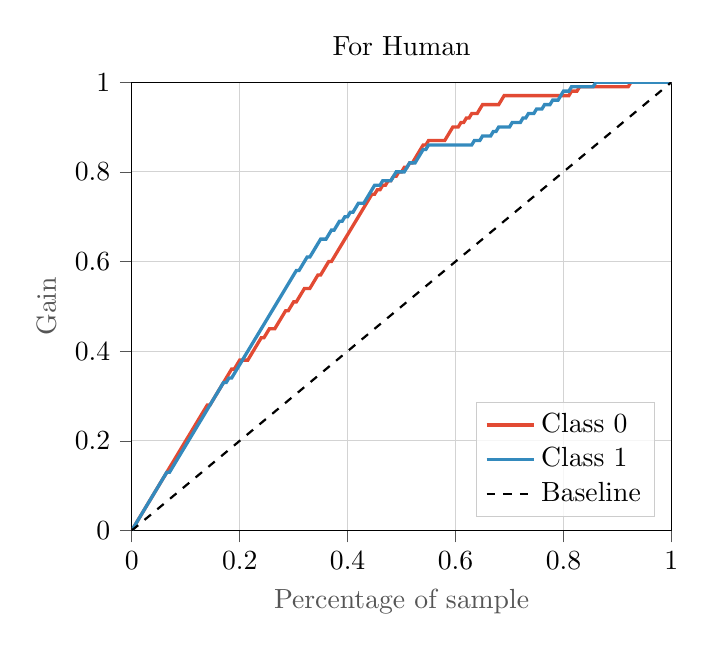
\begin{tikzpicture}

\definecolor{chocolate2267451}{RGB}{226,74,51}
\definecolor{dimgray85}{RGB}{85,85,85}
\definecolor{lightgray}{RGB}{211,211,211}
\definecolor{lightgray204}{RGB}{204,204,204}
\definecolor{steelblue52138189}{RGB}{52,138,189}

\begin{axis}[
legend cell align={left},
legend style={
  fill opacity=0.8,
  draw opacity=1,
  text opacity=1,
  at={(0.97,0.03)},
  anchor=south east,
  draw=lightgray204
},
tick align=outside,
tick pos=left,
title={For Human},
x grid style={lightgray},
xlabel=\textcolor{dimgray85}{Percentage of sample},
xmajorgrids,
xmin=0, xmax=1,
xtick style={color=dimgray85},
y grid style={lightgray},
ylabel=\textcolor{dimgray85}{Gain},
ymajorgrids,
ymin=0, ymax=1,
ytick style={color=dimgray85}
]
\addplot [very thick, chocolate2267451]
table {%
0 0
0.005 0.01
0.01 0.02
0.015 0.03
0.02 0.04
0.025 0.05
0.03 0.06
0.035 0.07
0.04 0.08
0.045 0.09
0.05 0.1
0.055 0.11
0.06 0.12
0.065 0.13
0.07 0.14
0.075 0.15
0.08 0.16
0.085 0.17
0.09 0.18
0.095 0.19
0.1 0.2
0.105 0.21
0.11 0.22
0.115 0.23
0.12 0.24
0.125 0.25
0.13 0.26
0.135 0.27
0.14 0.28
0.145 0.28
0.15 0.29
0.155 0.3
0.16 0.31
0.165 0.32
0.17 0.33
0.175 0.34
0.18 0.35
0.185 0.36
0.19 0.36
0.195 0.37
0.2 0.38
0.205 0.38
0.21 0.38
0.215 0.38
0.22 0.39
0.225 0.4
0.23 0.41
0.235 0.42
0.24 0.43
0.245 0.43
0.25 0.44
0.255 0.45
0.26 0.45
0.265 0.45
0.27 0.46
0.275 0.47
0.28 0.48
0.285 0.49
0.29 0.49
0.295 0.5
0.3 0.51
0.305 0.51
0.31 0.52
0.315 0.53
0.32 0.54
0.325 0.54
0.33 0.54
0.335 0.55
0.34 0.56
0.345 0.57
0.35 0.57
0.355 0.58
0.36 0.59
0.365 0.6
0.37 0.6
0.375 0.61
0.38 0.62
0.385 0.63
0.39 0.64
0.395 0.65
0.4 0.66
0.405 0.67
0.41 0.68
0.415 0.69
0.42 0.7
0.425 0.71
0.43 0.72
0.435 0.73
0.44 0.74
0.445 0.75
0.45 0.75
0.455 0.76
0.46 0.76
0.465 0.77
0.47 0.77
0.475 0.78
0.48 0.78
0.485 0.79
0.49 0.79
0.495 0.8
0.5 0.8
0.505 0.81
0.51 0.81
0.515 0.82
0.52 0.82
0.525 0.83
0.53 0.84
0.535 0.85
0.54 0.86
0.545 0.86
0.55 0.87
0.555 0.87
0.56 0.87
0.565 0.87
0.57 0.87
0.575 0.87
0.58 0.87
0.585 0.88
0.59 0.89
0.595 0.9
0.6 0.9
0.605 0.9
0.61 0.91
0.615 0.91
0.62 0.92
0.625 0.92
0.63 0.93
0.635 0.93
0.64 0.93
0.645 0.94
0.65 0.95
0.655 0.95
0.66 0.95
0.665 0.95
0.67 0.95
0.675 0.95
0.68 0.95
0.685 0.96
0.69 0.97
0.695 0.97
0.7 0.97
0.705 0.97
0.71 0.97
0.715 0.97
0.72 0.97
0.725 0.97
0.73 0.97
0.735 0.97
0.74 0.97
0.745 0.97
0.75 0.97
0.755 0.97
0.76 0.97
0.765 0.97
0.77 0.97
0.775 0.97
0.78 0.97
0.785 0.97
0.79 0.97
0.795 0.97
0.8 0.97
0.805 0.97
0.81 0.97
0.815 0.98
0.82 0.98
0.825 0.98
0.83 0.99
0.835 0.99
0.84 0.99
0.845 0.99
0.85 0.99
0.855 0.99
0.86 0.99
0.865 0.99
0.87 0.99
0.875 0.99
0.88 0.99
0.885 0.99
0.89 0.99
0.895 0.99
0.9 0.99
0.905 0.99
0.91 0.99
0.915 0.99
0.92 0.99
0.925 1
0.93 1
0.935 1
0.94 1
0.945 1
0.95 1
0.955 1
0.96 1
0.965 1
0.97 1
0.975 1
0.98 1
0.985 1
0.99 1
0.995 1
1 1
};
\addlegendentry{Class 0}
\addplot [very thick, steelblue52138189]
table {%
0 0
0.005 0.01
0.01 0.02
0.015 0.03
0.02 0.04
0.025 0.05
0.03 0.06
0.035 0.07
0.04 0.08
0.045 0.09
0.05 0.1
0.055 0.11
0.06 0.12
0.065 0.13
0.07 0.13
0.075 0.14
0.08 0.15
0.085 0.16
0.09 0.17
0.095 0.18
0.1 0.19
0.105 0.2
0.11 0.21
0.115 0.22
0.12 0.23
0.125 0.24
0.13 0.25
0.135 0.26
0.14 0.27
0.145 0.28
0.15 0.29
0.155 0.3
0.16 0.31
0.165 0.32
0.17 0.33
0.175 0.33
0.18 0.34
0.185 0.34
0.19 0.35
0.195 0.36
0.2 0.37
0.205 0.38
0.21 0.39
0.215 0.4
0.22 0.41
0.225 0.42
0.23 0.43
0.235 0.44
0.24 0.45
0.245 0.46
0.25 0.47
0.255 0.48
0.26 0.49
0.265 0.5
0.27 0.51
0.275 0.52
0.28 0.53
0.285 0.54
0.29 0.55
0.295 0.56
0.3 0.57
0.305 0.58
0.31 0.58
0.315 0.59
0.32 0.6
0.325 0.61
0.33 0.61
0.335 0.62
0.34 0.63
0.345 0.64
0.35 0.65
0.355 0.65
0.36 0.65
0.365 0.66
0.37 0.67
0.375 0.67
0.38 0.68
0.385 0.69
0.39 0.69
0.395 0.7
0.4 0.7
0.405 0.71
0.41 0.71
0.415 0.72
0.42 0.73
0.425 0.73
0.43 0.73
0.435 0.74
0.44 0.75
0.445 0.76
0.45 0.77
0.455 0.77
0.46 0.77
0.465 0.78
0.47 0.78
0.475 0.78
0.48 0.78
0.485 0.79
0.49 0.8
0.495 0.8
0.5 0.8
0.505 0.8
0.51 0.81
0.515 0.82
0.52 0.82
0.525 0.82
0.53 0.83
0.535 0.84
0.54 0.85
0.545 0.85
0.55 0.86
0.555 0.86
0.56 0.86
0.565 0.86
0.57 0.86
0.575 0.86
0.58 0.86
0.585 0.86
0.59 0.86
0.595 0.86
0.6 0.86
0.605 0.86
0.61 0.86
0.615 0.86
0.62 0.86
0.625 0.86
0.63 0.86
0.635 0.87
0.64 0.87
0.645 0.87
0.65 0.88
0.655 0.88
0.66 0.88
0.665 0.88
0.67 0.89
0.675 0.89
0.68 0.9
0.685 0.9
0.69 0.9
0.695 0.9
0.7 0.9
0.705 0.91
0.71 0.91
0.715 0.91
0.72 0.91
0.725 0.92
0.73 0.92
0.735 0.93
0.74 0.93
0.745 0.93
0.75 0.94
0.755 0.94
0.76 0.94
0.765 0.95
0.77 0.95
0.775 0.95
0.78 0.96
0.785 0.96
0.79 0.96
0.795 0.97
0.8 0.98
0.805 0.98
0.81 0.98
0.815 0.99
0.82 0.99
0.825 0.99
0.83 0.99
0.835 0.99
0.84 0.99
0.845 0.99
0.85 0.99
0.855 0.99
0.86 1
0.865 1
0.87 1
0.875 1
0.88 1
0.885 1
0.89 1
0.895 1
0.9 1
0.905 1
0.91 1
0.915 1
0.92 1
0.925 1
0.93 1
0.935 1
0.94 1
0.945 1
0.95 1
0.955 1
0.96 1
0.965 1
0.97 1
0.975 1
0.98 1
0.985 1
0.99 1
0.995 1
1 1
};
\addlegendentry{Class 1}
\addplot [thick, black, dashed]
table {%
0 0
1 1
};
\addlegendentry{Baseline}
\end{axis}

\end{tikzpicture}
&% This file was created with tikzplotlib v0.10.1.
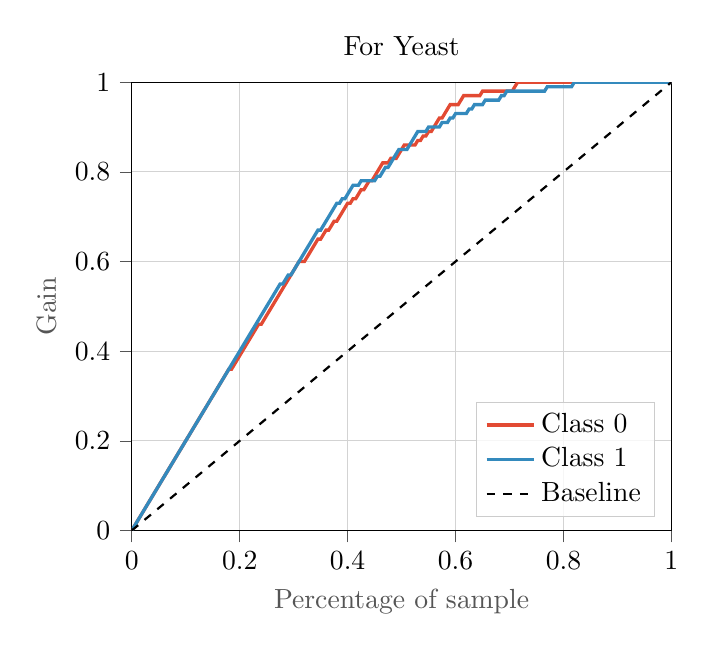
\begin{tikzpicture}

\definecolor{chocolate2267451}{RGB}{226,74,51}
\definecolor{dimgray85}{RGB}{85,85,85}
\definecolor{lightgray}{RGB}{211,211,211}
\definecolor{lightgray204}{RGB}{204,204,204}
\definecolor{steelblue52138189}{RGB}{52,138,189}

\begin{axis}[
legend cell align={left},
legend style={
  fill opacity=0.8,
  draw opacity=1,
  text opacity=1,
  at={(0.97,0.03)},
  anchor=south east,
  draw=lightgray204
},
tick align=outside,
tick pos=left,
title={For Yeast},
x grid style={lightgray},
xlabel=\textcolor{dimgray85}{Percentage of sample},
xmajorgrids,
xmin=0, xmax=1,
xtick style={color=dimgray85},
y grid style={lightgray},
ylabel=\textcolor{dimgray85}{Gain},
ymajorgrids,
ymin=0, ymax=1,
ytick style={color=dimgray85}
]
\addplot [very thick, chocolate2267451]
table {%
0 0
0.005 0.01
0.01 0.02
0.015 0.03
0.02 0.04
0.025 0.05
0.03 0.06
0.035 0.07
0.04 0.08
0.045 0.09
0.05 0.1
0.055 0.11
0.06 0.12
0.065 0.13
0.07 0.14
0.075 0.15
0.08 0.16
0.085 0.17
0.09 0.18
0.095 0.19
0.1 0.2
0.105 0.21
0.11 0.22
0.115 0.23
0.12 0.24
0.125 0.25
0.13 0.26
0.135 0.27
0.14 0.28
0.145 0.29
0.15 0.3
0.155 0.31
0.16 0.32
0.165 0.33
0.17 0.34
0.175 0.35
0.18 0.36
0.185 0.36
0.19 0.37
0.195 0.38
0.2 0.39
0.205 0.4
0.21 0.41
0.215 0.42
0.22 0.43
0.225 0.44
0.23 0.45
0.235 0.46
0.24 0.46
0.245 0.47
0.25 0.48
0.255 0.49
0.26 0.5
0.265 0.51
0.27 0.52
0.275 0.53
0.28 0.54
0.285 0.55
0.29 0.56
0.295 0.57
0.3 0.58
0.305 0.59
0.31 0.6
0.315 0.6
0.32 0.6
0.325 0.61
0.33 0.62
0.335 0.63
0.34 0.64
0.345 0.65
0.35 0.65
0.355 0.66
0.36 0.67
0.365 0.67
0.37 0.68
0.375 0.69
0.38 0.69
0.385 0.7
0.39 0.71
0.395 0.72
0.4 0.73
0.405 0.73
0.41 0.74
0.415 0.74
0.42 0.75
0.425 0.76
0.43 0.76
0.435 0.77
0.44 0.78
0.445 0.78
0.45 0.79
0.455 0.8
0.46 0.81
0.465 0.82
0.47 0.82
0.475 0.82
0.48 0.83
0.485 0.83
0.49 0.83
0.495 0.84
0.5 0.85
0.505 0.86
0.51 0.86
0.515 0.86
0.52 0.86
0.525 0.86
0.53 0.87
0.535 0.87
0.54 0.88
0.545 0.88
0.55 0.89
0.555 0.89
0.56 0.9
0.565 0.91
0.57 0.92
0.575 0.92
0.58 0.93
0.585 0.94
0.59 0.95
0.595 0.95
0.6 0.95
0.605 0.95
0.61 0.96
0.615 0.97
0.62 0.97
0.625 0.97
0.63 0.97
0.635 0.97
0.64 0.97
0.645 0.97
0.65 0.98
0.655 0.98
0.66 0.98
0.665 0.98
0.67 0.98
0.675 0.98
0.68 0.98
0.685 0.98
0.69 0.98
0.695 0.98
0.7 0.98
0.705 0.98
0.71 0.99
0.715 1
0.72 1
0.725 1
0.73 1
0.735 1
0.74 1
0.745 1
0.75 1
0.755 1
0.76 1
0.765 1
0.77 1
0.775 1
0.78 1
0.785 1
0.79 1
0.795 1
0.8 1
0.805 1
0.81 1
0.815 1
0.82 1
0.825 1
0.83 1
0.835 1
0.84 1
0.845 1
0.85 1
0.855 1
0.86 1
0.865 1
0.87 1
0.875 1
0.88 1
0.885 1
0.89 1
0.895 1
0.9 1
0.905 1
0.91 1
0.915 1
0.92 1
0.925 1
0.93 1
0.935 1
0.94 1
0.945 1
0.95 1
0.955 1
0.96 1
0.965 1
0.97 1
0.975 1
0.98 1
0.985 1
0.99 1
0.995 1
1 1
};
\addlegendentry{Class 0}
\addplot [very thick, steelblue52138189]
table {%
0 0
0.005 0.01
0.01 0.02
0.015 0.03
0.02 0.04
0.025 0.05
0.03 0.06
0.035 0.07
0.04 0.08
0.045 0.09
0.05 0.1
0.055 0.11
0.06 0.12
0.065 0.13
0.07 0.14
0.075 0.15
0.08 0.16
0.085 0.17
0.09 0.18
0.095 0.19
0.1 0.2
0.105 0.21
0.11 0.22
0.115 0.23
0.12 0.24
0.125 0.25
0.13 0.26
0.135 0.27
0.14 0.28
0.145 0.29
0.15 0.3
0.155 0.31
0.16 0.32
0.165 0.33
0.17 0.34
0.175 0.35
0.18 0.36
0.185 0.37
0.19 0.38
0.195 0.39
0.2 0.4
0.205 0.41
0.21 0.42
0.215 0.43
0.22 0.44
0.225 0.45
0.23 0.46
0.235 0.47
0.24 0.48
0.245 0.49
0.25 0.5
0.255 0.51
0.26 0.52
0.265 0.53
0.27 0.54
0.275 0.55
0.28 0.55
0.285 0.56
0.29 0.57
0.295 0.57
0.3 0.58
0.305 0.59
0.31 0.6
0.315 0.61
0.32 0.62
0.325 0.63
0.33 0.64
0.335 0.65
0.34 0.66
0.345 0.67
0.35 0.67
0.355 0.68
0.36 0.69
0.365 0.7
0.37 0.71
0.375 0.72
0.38 0.73
0.385 0.73
0.39 0.74
0.395 0.74
0.4 0.75
0.405 0.76
0.41 0.77
0.415 0.77
0.42 0.77
0.425 0.78
0.43 0.78
0.435 0.78
0.44 0.78
0.445 0.78
0.45 0.78
0.455 0.79
0.46 0.79
0.465 0.8
0.47 0.81
0.475 0.81
0.48 0.82
0.485 0.83
0.49 0.84
0.495 0.85
0.5 0.85
0.505 0.85
0.51 0.85
0.515 0.86
0.52 0.87
0.525 0.88
0.53 0.89
0.535 0.89
0.54 0.89
0.545 0.89
0.55 0.9
0.555 0.9
0.56 0.9
0.565 0.9
0.57 0.9
0.575 0.91
0.58 0.91
0.585 0.91
0.59 0.92
0.595 0.92
0.6 0.93
0.605 0.93
0.61 0.93
0.615 0.93
0.62 0.93
0.625 0.94
0.63 0.94
0.635 0.95
0.64 0.95
0.645 0.95
0.65 0.95
0.655 0.96
0.66 0.96
0.665 0.96
0.67 0.96
0.675 0.96
0.68 0.96
0.685 0.97
0.69 0.97
0.695 0.98
0.7 0.98
0.705 0.98
0.71 0.98
0.715 0.98
0.72 0.98
0.725 0.98
0.73 0.98
0.735 0.98
0.74 0.98
0.745 0.98
0.75 0.98
0.755 0.98
0.76 0.98
0.765 0.98
0.77 0.99
0.775 0.99
0.78 0.99
0.785 0.99
0.79 0.99
0.795 0.99
0.8 0.99
0.805 0.99
0.81 0.99
0.815 0.99
0.82 1
0.825 1
0.83 1
0.835 1
0.84 1
0.845 1
0.85 1
0.855 1
0.86 1
0.865 1
0.87 1
0.875 1
0.88 1
0.885 1
0.89 1
0.895 1
0.9 1
0.905 1
0.91 1
0.915 1
0.92 1
0.925 1
0.93 1
0.935 1
0.94 1
0.945 1
0.95 1
0.955 1
0.96 1
0.965 1
0.97 1
0.975 1
0.98 1
0.985 1
0.99 1
0.995 1
1 1
};
\addlegendentry{Class 1}
\addplot [thick, black, dashed]
table {%
0 0
1 1
};
\addlegendentry{Baseline}
\end{axis}

\end{tikzpicture}
 \\
  \end{tabular}
  \caption{Cumulative Gain Charts}
\end{table}


\begin{table}
  \begin{tabular}{ccc}
    % This file was created with tikzplotlib v0.10.1.
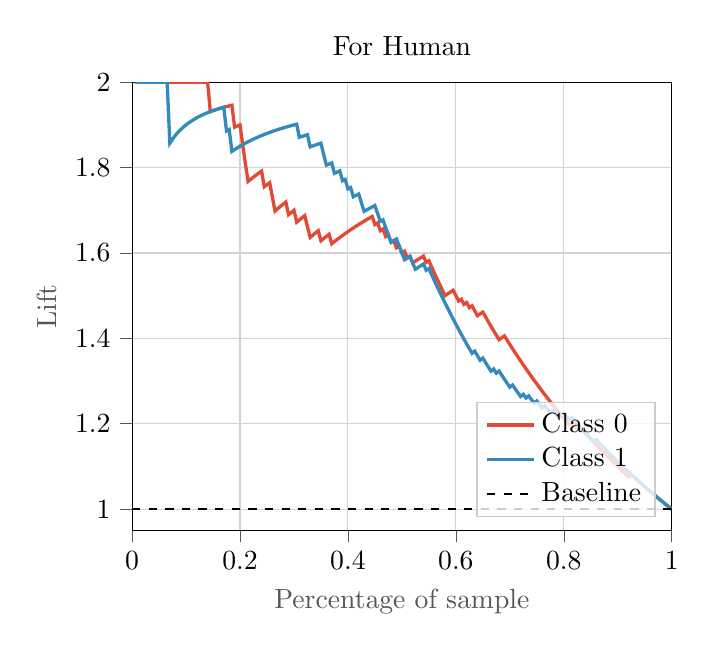
\begin{tikzpicture}

\definecolor{chocolate2267451}{RGB}{226,74,51}
\definecolor{dimgray85}{RGB}{85,85,85}
\definecolor{lightgray}{RGB}{211,211,211}
\definecolor{lightgray204}{RGB}{204,204,204}
\definecolor{steelblue52138189}{RGB}{52,138,189}

\begin{axis}[
legend cell align={left},
legend style={
  fill opacity=0.8,
  draw opacity=1,
  text opacity=1,
  at={(0.97,0.03)},
  anchor=south east,
  draw=lightgray204
},
tick align=outside,
tick pos=left,
title={For Human},
x grid style={lightgray},
xlabel=\textcolor{dimgray85}{Percentage of sample},
xmajorgrids,
xmin=0, xmax=1,
xtick style={color=dimgray85},
y grid style={lightgray},
ylabel=\textcolor{dimgray85}{Lift},
ymajorgrids,
ymin=0.95, ymax=2,
ytick style={color=dimgray85}
]
\addplot [very thick, chocolate2267451]
table {%
0.005 2
0.01 2
0.015 2
0.02 2
0.025 2
0.03 2
0.035 2
0.04 2
0.045 2
0.05 2
0.055 2
0.06 2
0.065 2
0.07 2
0.075 2
0.08 2
0.085 2
0.09 2
0.095 2
0.1 2
0.105 2
0.11 2
0.115 2
0.12 2
0.125 2
0.13 2
0.135 2
0.14 2
0.145 1.93103448275862
0.15 1.93333333333333
0.155 1.93548387096774
0.16 1.9375
0.165 1.93939393939394
0.17 1.94117647058824
0.175 1.94285714285714
0.18 1.94444444444444
0.185 1.94594594594595
0.19 1.89473684210526
0.195 1.8974358974359
0.2 1.9
0.205 1.85365853658537
0.21 1.80952380952381
0.215 1.76744186046512
0.22 1.77272727272727
0.225 1.77777777777778
0.23 1.78260869565217
0.235 1.78723404255319
0.24 1.79166666666667
0.245 1.75510204081633
0.25 1.76
0.255 1.76470588235294
0.26 1.73076923076923
0.265 1.69811320754717
0.27 1.7037037037037
0.275 1.70909090909091
0.28 1.71428571428571
0.285 1.71929824561404
0.29 1.68965517241379
0.295 1.69491525423729
0.3 1.7
0.305 1.67213114754098
0.31 1.67741935483871
0.315 1.68253968253968
0.32 1.6875
0.325 1.66153846153846
0.33 1.63636363636364
0.335 1.64179104477612
0.34 1.64705882352941
0.345 1.65217391304348
0.35 1.62857142857143
0.355 1.63380281690141
0.36 1.63888888888889
0.365 1.64383561643836
0.37 1.62162162162162
0.375 1.62666666666667
0.38 1.63157894736842
0.385 1.63636363636364
0.39 1.64102564102564
0.395 1.64556962025316
0.4 1.65
0.405 1.65432098765432
0.41 1.65853658536585
0.415 1.66265060240964
0.42 1.66666666666667
0.425 1.67058823529412
0.43 1.67441860465116
0.435 1.67816091954023
0.44 1.68181818181818
0.445 1.68539325842697
0.45 1.66666666666667
0.455 1.67032967032967
0.46 1.65217391304348
0.465 1.65591397849462
0.47 1.63829787234043
0.475 1.64210526315789
0.48 1.625
0.485 1.62886597938144
0.49 1.61224489795918
0.495 1.61616161616162
0.5 1.6
0.505 1.6039603960396
0.51 1.58823529411765
0.515 1.59223300970874
0.52 1.57692307692308
0.525 1.58095238095238
0.53 1.58490566037736
0.535 1.58878504672897
0.54 1.59259259259259
0.545 1.57798165137615
0.55 1.58181818181818
0.555 1.56756756756757
0.56 1.55357142857143
0.565 1.53982300884956
0.57 1.52631578947368
0.575 1.51304347826087
0.58 1.5
0.585 1.5042735042735
0.59 1.50847457627119
0.595 1.51260504201681
0.6 1.5
0.605 1.48760330578512
0.61 1.49180327868852
0.615 1.47967479674797
0.62 1.48387096774194
0.625 1.472
0.63 1.47619047619048
0.635 1.46456692913386
0.64 1.453125
0.645 1.45736434108527
0.65 1.46153846153846
0.655 1.45038167938931
0.66 1.43939393939394
0.665 1.42857142857143
0.67 1.41791044776119
0.675 1.40740740740741
0.68 1.39705882352941
0.685 1.4014598540146
0.69 1.40579710144928
0.695 1.39568345323741
0.7 1.38571428571429
0.705 1.3758865248227
0.71 1.36619718309859
0.715 1.35664335664336
0.72 1.34722222222222
0.725 1.33793103448276
0.73 1.32876712328767
0.735 1.31972789115646
0.74 1.31081081081081
0.745 1.30201342281879
0.75 1.29333333333333
0.755 1.28476821192053
0.76 1.27631578947368
0.765 1.26797385620915
0.77 1.25974025974026
0.775 1.25161290322581
0.78 1.24358974358974
0.785 1.23566878980892
0.79 1.22784810126582
0.795 1.22012578616352
0.8 1.2125
0.805 1.20496894409938
0.81 1.19753086419753
0.815 1.20245398773006
0.82 1.19512195121951
0.825 1.18787878787879
0.83 1.19277108433735
0.835 1.18562874251497
0.84 1.17857142857143
0.845 1.17159763313609
0.85 1.16470588235294
0.855 1.15789473684211
0.86 1.15116279069767
0.865 1.14450867052023
0.87 1.13793103448276
0.875 1.13142857142857
0.88 1.125
0.885 1.11864406779661
0.89 1.1123595505618
0.895 1.10614525139665
0.9 1.1
0.905 1.0939226519337
0.91 1.08791208791209
0.915 1.08196721311475
0.92 1.07608695652174
0.925 1.08108108108108
0.93 1.0752688172043
0.935 1.06951871657754
0.94 1.06382978723404
0.945 1.05820105820106
0.95 1.05263157894737
0.955 1.04712041884817
0.96 1.04166666666667
0.965 1.03626943005181
0.97 1.03092783505155
0.975 1.02564102564103
0.98 1.02040816326531
0.985 1.01522842639594
0.99 1.01010101010101
0.995 1.00502512562814
1 1
};
\addlegendentry{Class 0}
\addplot [very thick, steelblue52138189]
table {%
0.005 2
0.01 2
0.015 2
0.02 2
0.025 2
0.03 2
0.035 2
0.04 2
0.045 2
0.05 2
0.055 2
0.06 2
0.065 2
0.07 1.85714285714286
0.075 1.86666666666667
0.08 1.875
0.085 1.88235294117647
0.09 1.88888888888889
0.095 1.89473684210526
0.1 1.9
0.105 1.9047619047619
0.11 1.90909090909091
0.115 1.91304347826087
0.12 1.91666666666667
0.125 1.92
0.13 1.92307692307692
0.135 1.92592592592593
0.14 1.92857142857143
0.145 1.93103448275862
0.15 1.93333333333333
0.155 1.93548387096774
0.16 1.9375
0.165 1.93939393939394
0.17 1.94117647058824
0.175 1.88571428571429
0.18 1.88888888888889
0.185 1.83783783783784
0.19 1.84210526315789
0.195 1.84615384615385
0.2 1.85
0.205 1.85365853658537
0.21 1.85714285714286
0.215 1.86046511627907
0.22 1.86363636363636
0.225 1.86666666666667
0.23 1.8695652173913
0.235 1.87234042553191
0.24 1.875
0.245 1.87755102040816
0.25 1.88
0.255 1.88235294117647
0.26 1.88461538461538
0.265 1.88679245283019
0.27 1.88888888888889
0.275 1.89090909090909
0.28 1.89285714285714
0.285 1.89473684210526
0.29 1.89655172413793
0.295 1.89830508474576
0.3 1.9
0.305 1.90163934426229
0.31 1.87096774193548
0.315 1.87301587301587
0.32 1.875
0.325 1.87692307692308
0.33 1.84848484848485
0.335 1.85074626865672
0.34 1.85294117647059
0.345 1.85507246376812
0.35 1.85714285714286
0.355 1.83098591549296
0.36 1.80555555555556
0.365 1.80821917808219
0.37 1.81081081081081
0.375 1.78666666666667
0.38 1.78947368421053
0.385 1.79220779220779
0.39 1.76923076923077
0.395 1.77215189873418
0.4 1.75
0.405 1.75308641975309
0.41 1.73170731707317
0.415 1.73493975903614
0.42 1.73809523809524
0.425 1.71764705882353
0.43 1.69767441860465
0.435 1.70114942528736
0.44 1.70454545454545
0.445 1.70786516853933
0.45 1.71111111111111
0.455 1.69230769230769
0.46 1.67391304347826
0.465 1.67741935483871
0.47 1.65957446808511
0.475 1.64210526315789
0.48 1.625
0.485 1.62886597938144
0.49 1.63265306122449
0.495 1.61616161616162
0.5 1.6
0.505 1.58415841584158
0.51 1.58823529411765
0.515 1.59223300970874
0.52 1.57692307692308
0.525 1.56190476190476
0.53 1.56603773584906
0.535 1.57009345794393
0.54 1.57407407407407
0.545 1.55963302752294
0.55 1.56363636363636
0.555 1.54954954954955
0.56 1.53571428571429
0.565 1.52212389380531
0.57 1.50877192982456
0.575 1.49565217391304
0.58 1.48275862068966
0.585 1.47008547008547
0.59 1.45762711864407
0.595 1.4453781512605
0.6 1.43333333333333
0.605 1.42148760330579
0.61 1.40983606557377
0.615 1.39837398373984
0.62 1.38709677419355
0.625 1.376
0.63 1.36507936507937
0.635 1.37007874015748
0.64 1.359375
0.645 1.34883720930233
0.65 1.35384615384615
0.655 1.34351145038168
0.66 1.33333333333333
0.665 1.32330827067669
0.67 1.32835820895522
0.675 1.31851851851852
0.68 1.32352941176471
0.685 1.31386861313869
0.69 1.30434782608696
0.695 1.29496402877698
0.7 1.28571428571429
0.705 1.29078014184397
0.71 1.28169014084507
0.715 1.27272727272727
0.72 1.26388888888889
0.725 1.26896551724138
0.73 1.26027397260274
0.735 1.26530612244898
0.74 1.25675675675676
0.745 1.24832214765101
0.75 1.25333333333333
0.755 1.24503311258278
0.76 1.23684210526316
0.765 1.24183006535948
0.77 1.23376623376623
0.775 1.2258064516129
0.78 1.23076923076923
0.785 1.22292993630573
0.79 1.21518987341772
0.795 1.22012578616352
0.8 1.225
0.805 1.21739130434783
0.81 1.20987654320988
0.815 1.21472392638037
0.82 1.20731707317073
0.825 1.2
0.83 1.19277108433735
0.835 1.18562874251497
0.84 1.17857142857143
0.845 1.17159763313609
0.85 1.16470588235294
0.855 1.15789473684211
0.86 1.16279069767442
0.865 1.15606936416185
0.87 1.14942528735632
0.875 1.14285714285714
0.88 1.13636363636364
0.885 1.12994350282486
0.89 1.12359550561798
0.895 1.11731843575419
0.9 1.11111111111111
0.905 1.10497237569061
0.91 1.0989010989011
0.915 1.09289617486339
0.92 1.08695652173913
0.925 1.08108108108108
0.93 1.0752688172043
0.935 1.06951871657754
0.94 1.06382978723404
0.945 1.05820105820106
0.95 1.05263157894737
0.955 1.04712041884817
0.96 1.04166666666667
0.965 1.03626943005181
0.97 1.03092783505155
0.975 1.02564102564103
0.98 1.02040816326531
0.985 1.01522842639594
0.99 1.01010101010101
0.995 1.00502512562814
1 1
};
\addlegendentry{Class 1}
\addplot [thick, black, dashed]
table {%
0 1
1 1
};
\addlegendentry{Baseline}
\end{axis}

\end{tikzpicture}
&% This file was created with tikzplotlib v0.10.1.
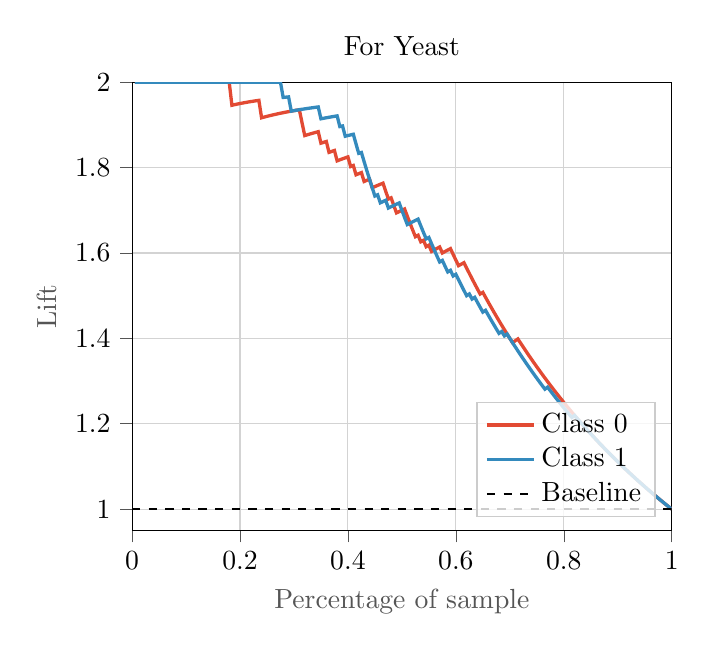
\begin{tikzpicture}

\definecolor{chocolate2267451}{RGB}{226,74,51}
\definecolor{dimgray85}{RGB}{85,85,85}
\definecolor{lightgray}{RGB}{211,211,211}
\definecolor{lightgray204}{RGB}{204,204,204}
\definecolor{steelblue52138189}{RGB}{52,138,189}

\begin{axis}[
legend cell align={left},
legend style={
  fill opacity=0.8,
  draw opacity=1,
  text opacity=1,
  at={(0.97,0.03)},
  anchor=south east,
  draw=lightgray204
},
tick align=outside,
tick pos=left,
title={For Yeast},
x grid style={lightgray},
xlabel=\textcolor{dimgray85}{Percentage of sample},
xmajorgrids,
xmin=0, xmax=1,
xtick style={color=dimgray85},
y grid style={lightgray},
ylabel=\textcolor{dimgray85}{Lift},
ymajorgrids,
ymin=0.95, ymax=2,
ytick style={color=dimgray85}
]
\addplot [very thick, chocolate2267451]
table {%
0.005 2
0.01 2
0.015 2
0.02 2
0.025 2
0.03 2
0.035 2
0.04 2
0.045 2
0.05 2
0.055 2
0.06 2
0.065 2
0.07 2
0.075 2
0.08 2
0.085 2
0.09 2
0.095 2
0.1 2
0.105 2
0.11 2
0.115 2
0.12 2
0.125 2
0.13 2
0.135 2
0.14 2
0.145 2
0.15 2
0.155 2
0.16 2
0.165 2
0.17 2
0.175 2
0.18 2
0.185 1.94594594594595
0.19 1.94736842105263
0.195 1.94871794871795
0.2 1.95
0.205 1.95121951219512
0.21 1.95238095238095
0.215 1.95348837209302
0.22 1.95454545454545
0.225 1.95555555555556
0.23 1.95652173913043
0.235 1.95744680851064
0.24 1.91666666666667
0.245 1.91836734693878
0.25 1.92
0.255 1.92156862745098
0.26 1.92307692307692
0.265 1.92452830188679
0.27 1.92592592592593
0.275 1.92727272727273
0.28 1.92857142857143
0.285 1.92982456140351
0.29 1.93103448275862
0.295 1.93220338983051
0.3 1.93333333333333
0.305 1.9344262295082
0.31 1.93548387096774
0.315 1.9047619047619
0.32 1.875
0.325 1.87692307692308
0.33 1.87878787878788
0.335 1.88059701492537
0.34 1.88235294117647
0.345 1.88405797101449
0.35 1.85714285714286
0.355 1.85915492957746
0.36 1.86111111111111
0.365 1.83561643835616
0.37 1.83783783783784
0.375 1.84
0.38 1.81578947368421
0.385 1.81818181818182
0.39 1.82051282051282
0.395 1.82278481012658
0.4 1.825
0.405 1.80246913580247
0.41 1.80487804878049
0.415 1.78313253012048
0.42 1.78571428571429
0.425 1.78823529411765
0.43 1.76744186046512
0.435 1.77011494252874
0.44 1.77272727272727
0.445 1.75280898876405
0.45 1.75555555555556
0.455 1.75824175824176
0.46 1.76086956521739
0.465 1.76344086021505
0.47 1.74468085106383
0.475 1.72631578947368
0.48 1.72916666666667
0.485 1.71134020618557
0.49 1.69387755102041
0.495 1.6969696969697
0.5 1.7
0.505 1.7029702970297
0.51 1.68627450980392
0.515 1.66990291262136
0.52 1.65384615384615
0.525 1.63809523809524
0.53 1.64150943396226
0.535 1.62616822429907
0.54 1.62962962962963
0.545 1.61467889908257
0.55 1.61818181818182
0.555 1.6036036036036
0.56 1.60714285714286
0.565 1.61061946902655
0.57 1.6140350877193
0.575 1.6
0.58 1.60344827586207
0.585 1.60683760683761
0.59 1.61016949152542
0.595 1.59663865546218
0.6 1.58333333333333
0.605 1.5702479338843
0.61 1.57377049180328
0.615 1.57723577235772
0.62 1.56451612903226
0.625 1.552
0.63 1.53968253968254
0.635 1.52755905511811
0.64 1.515625
0.645 1.50387596899225
0.65 1.50769230769231
0.655 1.49618320610687
0.66 1.48484848484848
0.665 1.47368421052632
0.67 1.46268656716418
0.675 1.45185185185185
0.68 1.44117647058824
0.685 1.43065693430657
0.69 1.42028985507246
0.695 1.41007194244604
0.7 1.4
0.705 1.39007092198582
0.71 1.3943661971831
0.715 1.3986013986014
0.72 1.38888888888889
0.725 1.37931034482759
0.73 1.36986301369863
0.735 1.36054421768707
0.74 1.35135135135135
0.745 1.34228187919463
0.75 1.33333333333333
0.755 1.32450331125828
0.76 1.31578947368421
0.765 1.30718954248366
0.77 1.2987012987013
0.775 1.29032258064516
0.78 1.28205128205128
0.785 1.27388535031847
0.79 1.26582278481013
0.795 1.25786163522013
0.8 1.25
0.805 1.24223602484472
0.81 1.23456790123457
0.815 1.22699386503067
0.82 1.21951219512195
0.825 1.21212121212121
0.83 1.20481927710843
0.835 1.19760479041916
0.84 1.19047619047619
0.845 1.18343195266272
0.85 1.17647058823529
0.855 1.16959064327485
0.86 1.16279069767442
0.865 1.15606936416185
0.87 1.14942528735632
0.875 1.14285714285714
0.88 1.13636363636364
0.885 1.12994350282486
0.89 1.12359550561798
0.895 1.11731843575419
0.9 1.11111111111111
0.905 1.10497237569061
0.91 1.0989010989011
0.915 1.09289617486339
0.92 1.08695652173913
0.925 1.08108108108108
0.93 1.0752688172043
0.935 1.06951871657754
0.94 1.06382978723404
0.945 1.05820105820106
0.95 1.05263157894737
0.955 1.04712041884817
0.96 1.04166666666667
0.965 1.03626943005181
0.97 1.03092783505155
0.975 1.02564102564103
0.98 1.02040816326531
0.985 1.01522842639594
0.99 1.01010101010101
0.995 1.00502512562814
1 1
};
\addlegendentry{Class 0}
\addplot [very thick, steelblue52138189]
table {%
0.005 2
0.01 2
0.015 2
0.02 2
0.025 2
0.03 2
0.035 2
0.04 2
0.045 2
0.05 2
0.055 2
0.06 2
0.065 2
0.07 2
0.075 2
0.08 2
0.085 2
0.09 2
0.095 2
0.1 2
0.105 2
0.11 2
0.115 2
0.12 2
0.125 2
0.13 2
0.135 2
0.14 2
0.145 2
0.15 2
0.155 2
0.16 2
0.165 2
0.17 2
0.175 2
0.18 2
0.185 2
0.19 2
0.195 2
0.2 2
0.205 2
0.21 2
0.215 2
0.22 2
0.225 2
0.23 2
0.235 2
0.24 2
0.245 2
0.25 2
0.255 2
0.26 2
0.265 2
0.27 2
0.275 2
0.28 1.96428571428571
0.285 1.96491228070175
0.29 1.96551724137931
0.295 1.93220338983051
0.3 1.93333333333333
0.305 1.9344262295082
0.31 1.93548387096774
0.315 1.93650793650794
0.32 1.9375
0.325 1.93846153846154
0.33 1.93939393939394
0.335 1.94029850746269
0.34 1.94117647058824
0.345 1.94202898550725
0.35 1.91428571428571
0.355 1.91549295774648
0.36 1.91666666666667
0.365 1.91780821917808
0.37 1.91891891891892
0.375 1.92
0.38 1.92105263157895
0.385 1.8961038961039
0.39 1.8974358974359
0.395 1.87341772151899
0.4 1.875
0.405 1.87654320987654
0.41 1.8780487804878
0.415 1.85542168674699
0.42 1.83333333333333
0.425 1.83529411764706
0.43 1.81395348837209
0.435 1.79310344827586
0.44 1.77272727272727
0.445 1.75280898876405
0.45 1.73333333333333
0.455 1.73626373626374
0.46 1.71739130434783
0.465 1.72043010752688
0.47 1.72340425531915
0.475 1.70526315789474
0.48 1.70833333333333
0.485 1.71134020618557
0.49 1.71428571428571
0.495 1.71717171717172
0.5 1.7
0.505 1.68316831683168
0.51 1.66666666666667
0.515 1.66990291262136
0.52 1.67307692307692
0.525 1.67619047619048
0.53 1.67924528301887
0.535 1.66355140186916
0.54 1.64814814814815
0.545 1.63302752293578
0.55 1.63636363636364
0.555 1.62162162162162
0.56 1.60714285714286
0.565 1.5929203539823
0.57 1.57894736842105
0.575 1.58260869565217
0.58 1.56896551724138
0.585 1.55555555555556
0.59 1.55932203389831
0.595 1.54621848739496
0.6 1.55
0.605 1.53719008264463
0.61 1.52459016393443
0.615 1.51219512195122
0.62 1.5
0.625 1.504
0.63 1.49206349206349
0.635 1.49606299212598
0.64 1.484375
0.645 1.47286821705426
0.65 1.46153846153846
0.655 1.46564885496183
0.66 1.45454545454545
0.665 1.44360902255639
0.67 1.43283582089552
0.675 1.42222222222222
0.68 1.41176470588235
0.685 1.41605839416058
0.69 1.40579710144928
0.695 1.41007194244604
0.7 1.4
0.705 1.39007092198582
0.71 1.38028169014085
0.715 1.37062937062937
0.72 1.36111111111111
0.725 1.35172413793103
0.73 1.34246575342466
0.735 1.33333333333333
0.74 1.32432432432432
0.745 1.31543624161074
0.75 1.30666666666667
0.755 1.29801324503311
0.76 1.28947368421053
0.765 1.28104575163399
0.77 1.28571428571429
0.775 1.27741935483871
0.78 1.26923076923077
0.785 1.26114649681529
0.79 1.25316455696203
0.795 1.24528301886792
0.8 1.2375
0.805 1.22981366459627
0.81 1.22222222222222
0.815 1.21472392638037
0.82 1.21951219512195
0.825 1.21212121212121
0.83 1.20481927710843
0.835 1.19760479041916
0.84 1.19047619047619
0.845 1.18343195266272
0.85 1.17647058823529
0.855 1.16959064327485
0.86 1.16279069767442
0.865 1.15606936416185
0.87 1.14942528735632
0.875 1.14285714285714
0.88 1.13636363636364
0.885 1.12994350282486
0.89 1.12359550561798
0.895 1.11731843575419
0.9 1.11111111111111
0.905 1.10497237569061
0.91 1.0989010989011
0.915 1.09289617486339
0.92 1.08695652173913
0.925 1.08108108108108
0.93 1.0752688172043
0.935 1.06951871657754
0.94 1.06382978723404
0.945 1.05820105820106
0.95 1.05263157894737
0.955 1.04712041884817
0.96 1.04166666666667
0.965 1.03626943005181
0.97 1.03092783505155
0.975 1.02564102564103
0.98 1.02040816326531
0.985 1.01522842639594
0.99 1.01010101010101
0.995 1.00502512562814
1 1
};
\addlegendentry{Class 1}
\addplot [thick, black, dashed]
table {%
0 1
1 1
};
\addlegendentry{Baseline}
\end{axis}

\end{tikzpicture}
 \\
  \end{tabular}
  \caption{Lift Curves}
\end{table}

\end{landscape}
\end{document}
